\section{Stokastisitet}
\subsection{Counting}
\begin{frame}
\begin{block}{Product Rule}
\begin{itemize}
\item Noe kan brytes ned i to aksjoner som kombineres med hverandre
\item For den ene finnes det $n_1$ muligheter, for den andre $n_2$
\item Det blir $n_1\cdot n_2$ kombinasjoner
\end{itemize}
\end{block}
\begin{block}{Eksempel}
\begin{itemize}
\item Det er to type maskiner som trenges
\item Den ene finnes 3 ganger, den andre 5 ganger
\item Hvor mange kombinasjoner maskintype 1, maskintype 2 finnes det?
\item $5\cdot 3=15$
\end{itemize}
\end{block}
\end{frame}

\begin{frame}
\begin{block}{Sum Rule}
\begin{itemize}
\item Noe kan gjøres på enten en av $n_1$ måter, eller en av $n_2$ måter
\item Det finnes ingen element som er både i $n_1$ og i $n_2$
\item Det blir $n_1+n_2$ muligheter å gjøre det
\end{itemize}
\end{block}
\begin{block}{Eksempel}
\begin{itemize}
\item En student skal velge masteroppgaven sin
\item Hun liker tre fagområder
\item I område $n_1$ finnes det 5 teamer, i $n_2$ 3 temaer, i område $n_3$ er det 8
\item Det er $5+3+8=16$ temaer å velge fra
\end{itemize}
\end{block}
\end{frame}

\begin{frame}
\begin{block}{Subtraction Rule}
\begin{itemize}
\item Ligner \textit{Sum rule}, men flere elementer er i flere grupper
\item Noe kan gjøres på enten en av $n_1$ måter, eller en av $n_2$ måter, men noen er i både $n_1$ og $n_2$
\item Det blir $n_1+n_2-felles(n_1,n_2)$ muligheter
\end{itemize}
\end{block}
\begin{block}{Eksempel}
\begin{itemize}
\item På fredag er det amerikansk-norsk folkefest
\item Det er 22 amerikanere og 18 nordmenn som meldte seg på
\item 3 av dem er både norsk og amerikansk
\item Det er $22+18-3=37$ personer som deltar
\end{itemize}
\end{block}
\end{frame}

\begin{frame}
\begin{block}{Division Rule}
\begin{itemize}
\item Det er $n$ måter å gjøre noe, men egentlig finnes det for hver måte minst $d$ lignende måter
\item Det blir da $n/d$ forskjellige muligheter
\end{itemize}
\end{block}
\begin{block}{Eksempel}
\begin{itemize}
\item I en fornøyelsespark for katter blir det talt 400 beiner. Mennesker og andre dyr har ikke lov å være i fornøyelsesparken
\item Hver katt har eksakt fire bein
\item Det betyr det er $400/4=100$ katter
\end{itemize}
\end{block}
\end{frame}

\subsection*{Kombinatorikk}
\begin{frame}{Permutasjon? Kombinasjon? Variasjon? Hæ?}
\begin{enumerate}
\item Blir alle elementer med?
	\begin{itemize}
	\item Ja: Permutasjon
	\item Nei: Variasjon eller Kombinasjon
	\end{itemize}
\item (Permutasjon, Kombinasjon) Er rekkefølgen viktig?
	\begin{itemize}
	\item Ja: Variasjon
	\item Nei: Kombinasjon
	\end{itemize}
\item Finnes det elementer flere ganger?
	\begin{itemize}
	\item Permutasjon uten repetisjon: $n!$
	\item Permutasjon med repetisjon: $\frac{n!}{r!\cdot s!\cdot t!}$
	\item Kombinasjon uten repetisjon: ${n \choose k}$
	\item Kombinasjon med repetisjon: $ {(n+k-1) \choose k}$
	\item Variasjon uten repetisjon: $\frac{n!}{(n-k)!}$
	\item Variasjon med repetisjon: $n^k$
	\end{itemize}
\end{enumerate}
\end{frame}

\begin{frame}{Eksempler}
\begin{block}{Eksempel 1}
\begin{itemize}
\item 7 personer må fotograferes. Hvor mange kombinasjoner finnes det å ordne dem på bildet?
\item Alle elementer blir med, ingen repetisjon 
\item Permutasjon uten repetisjon: $n!=7!=720$
\end{itemize}
\end{block}

\begin{block}{Eksempel 2}
\begin{itemize}
\item Hvor mange måter finnes det for å ordne bokstavene \textit{Mississippi}?
\item Alle elementer blir med, men repetisjon (permutasjon)
\item $\frac{n!}{r!\cdot s!\cdot t!} =  \frac{11!}{4!\cdot 4!\cdot 2!}=34650$
\end{itemize}
\end{block}
\end{frame}

\begin{frame}{Enda flere eksempler}
\begin{block}{Eksempel 3}
\begin{itemize}
\item Det er 7 personer og 3 tilfeldige av dem skal få en pris. Hvor mange kombinasjoner finnes det?
\item Ikke alle elementer blir med, ingen repetisjon, rekkefølgen ikke viktig 
\item Kombinasjon uten repetisjon: ${n \choose k}={7 \choose 3}=\frac{7!}{3!\cdot 4!}=35$
\end{itemize}
\end{block}

\begin{block}{Eksempel 4}
\begin{itemize}
\item Vi har 5 typer is og skal spise 3 av dem. Vi er opptatt av rekkefølgen for best smak.
\item Ikke ealle lementer blir med, rekkefølge viktig, med repetisjon
\item $n^k=5^3=125$
\end{itemize}
\end{block}
\end{frame}

\subsection*{Spørretid}
\begin{frame}{Spørsmål?}
    \begin{figure}
        \centering
        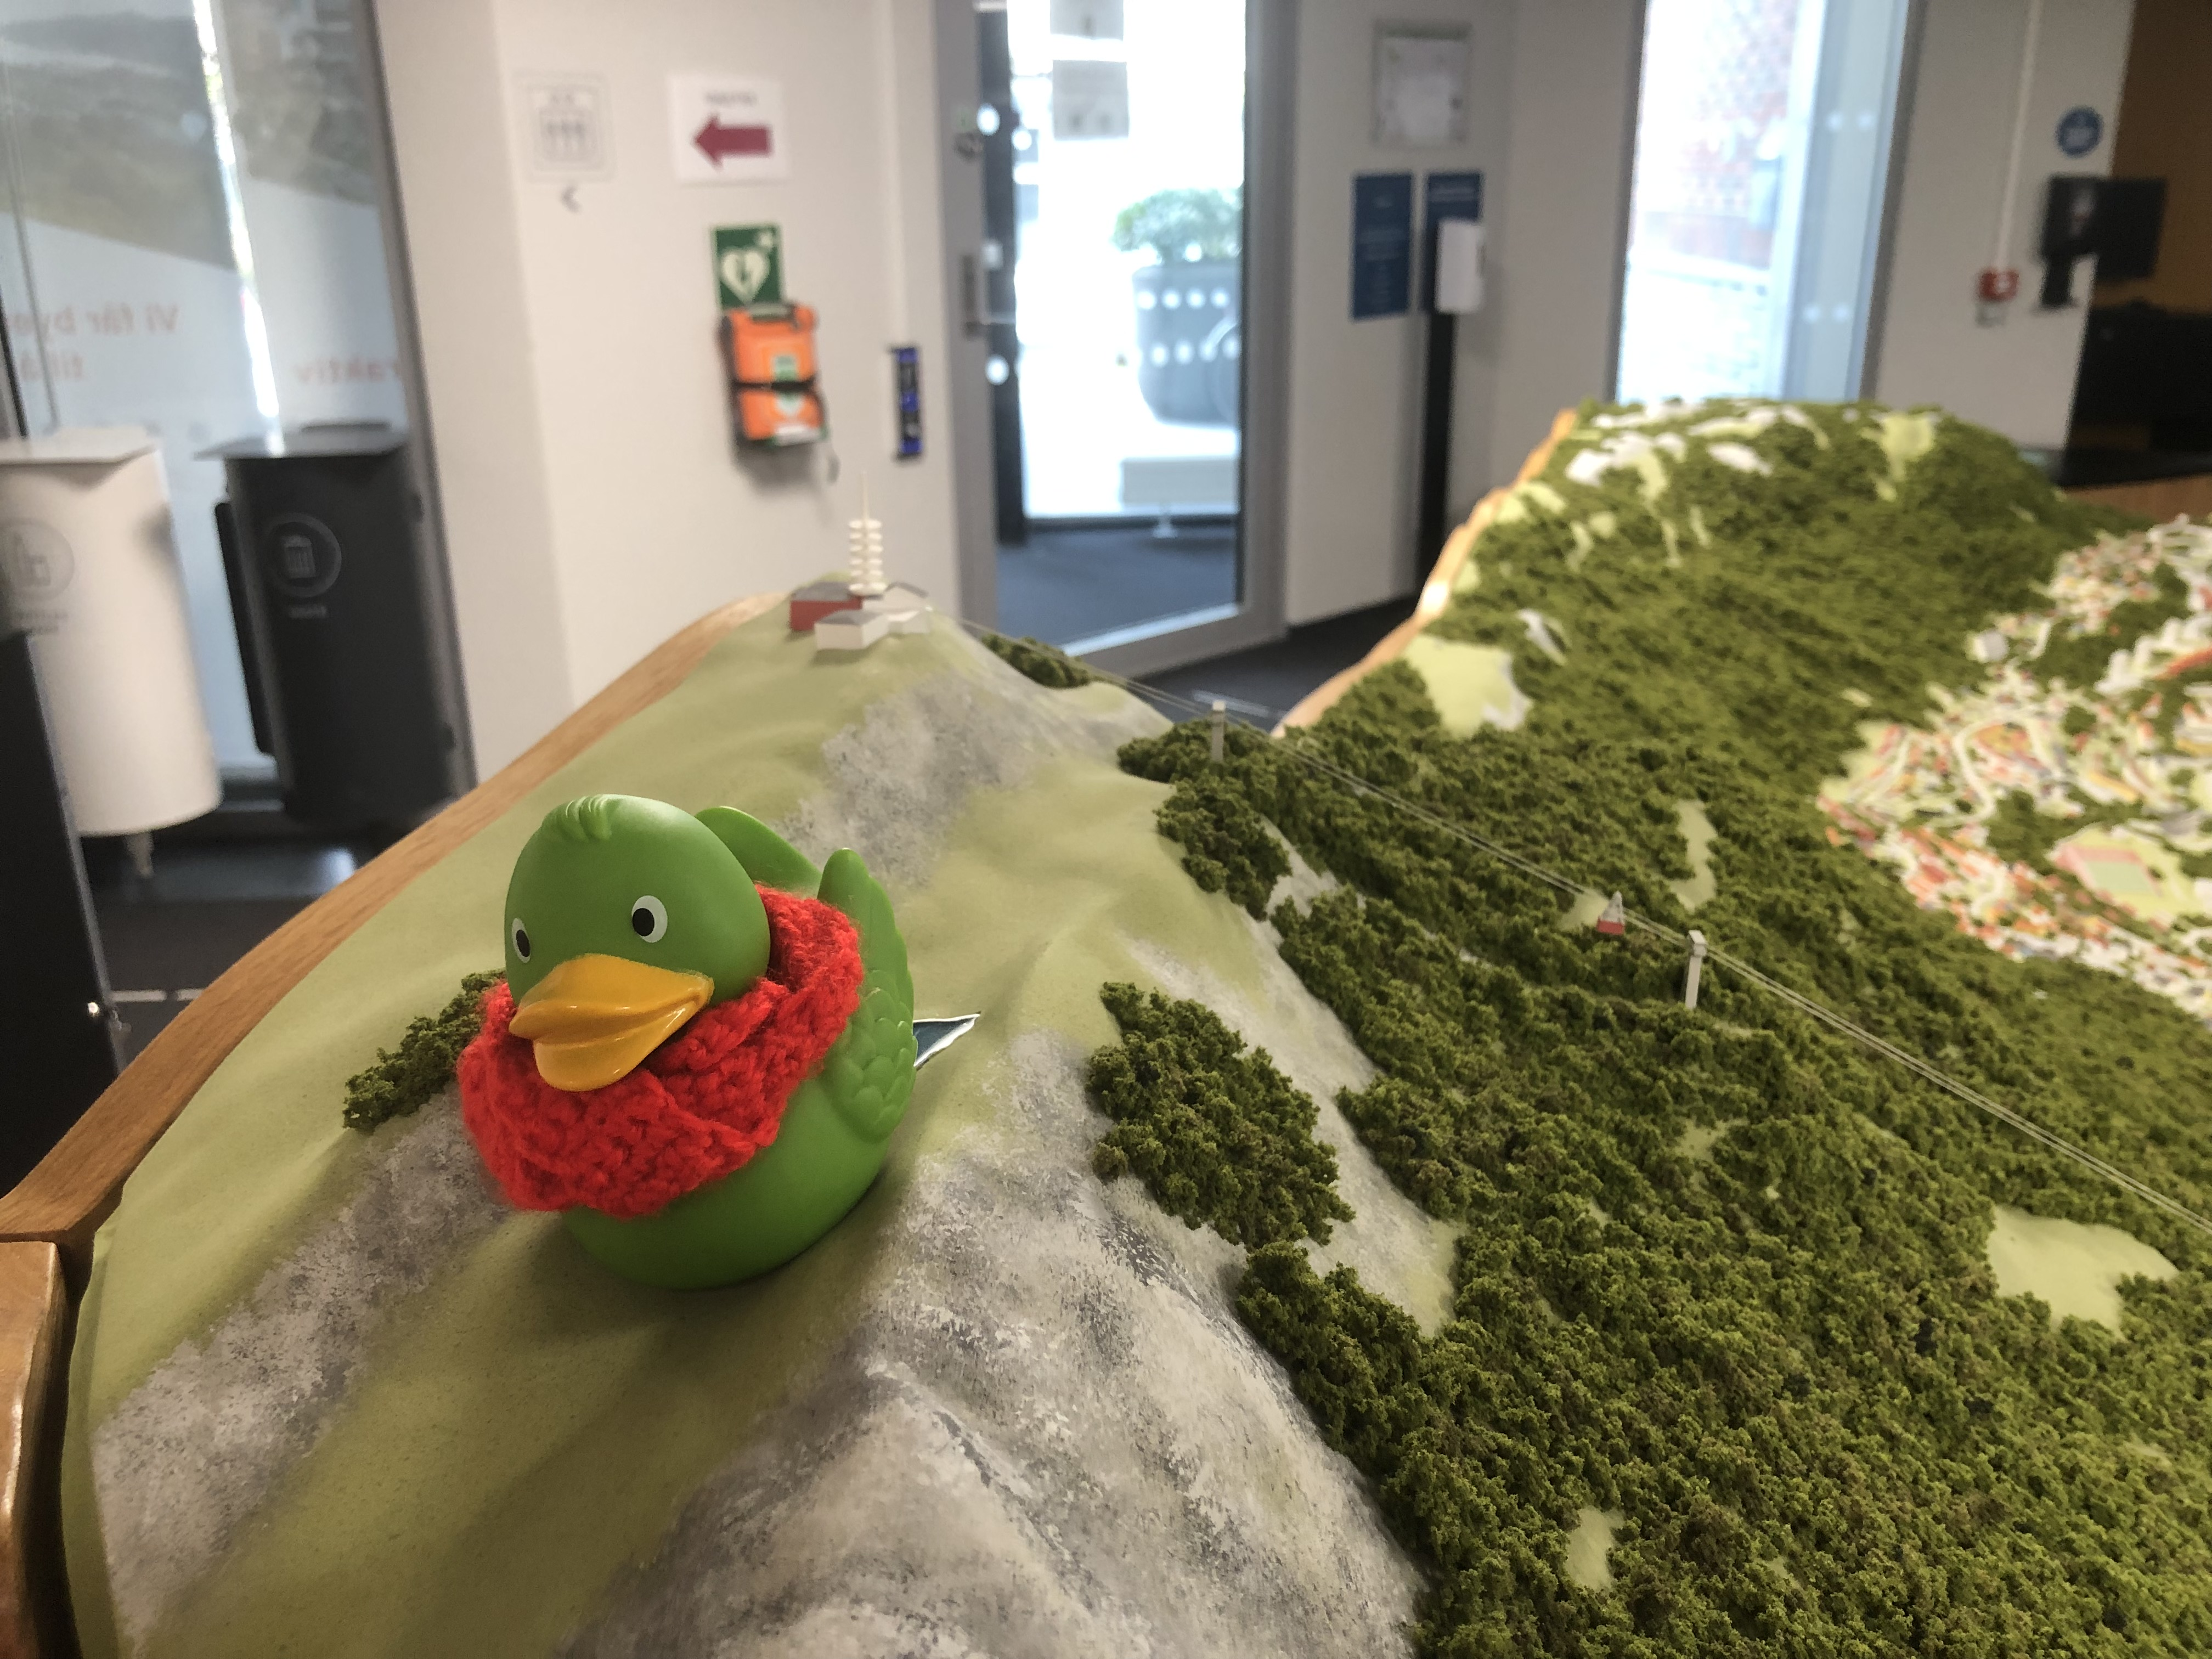
\includegraphics[height = 4.9cm]{images/guillaume11.jpg}
        \caption{Guillaume på Ulriken}
        \label{fig:guillaume11}
    \end{figure}
\end{frame}

\subsection{Sannsynligheter}
\begin{frame}
TODO: Fill with content @Lukas 
Bayes theorem, probabilitiy theory
discrete probability
expected value and variance
\end{frame}

\subsection*{Spørretid}
\begin{frame}{Spørsmål?}
    \begin{figure}
        \centering
        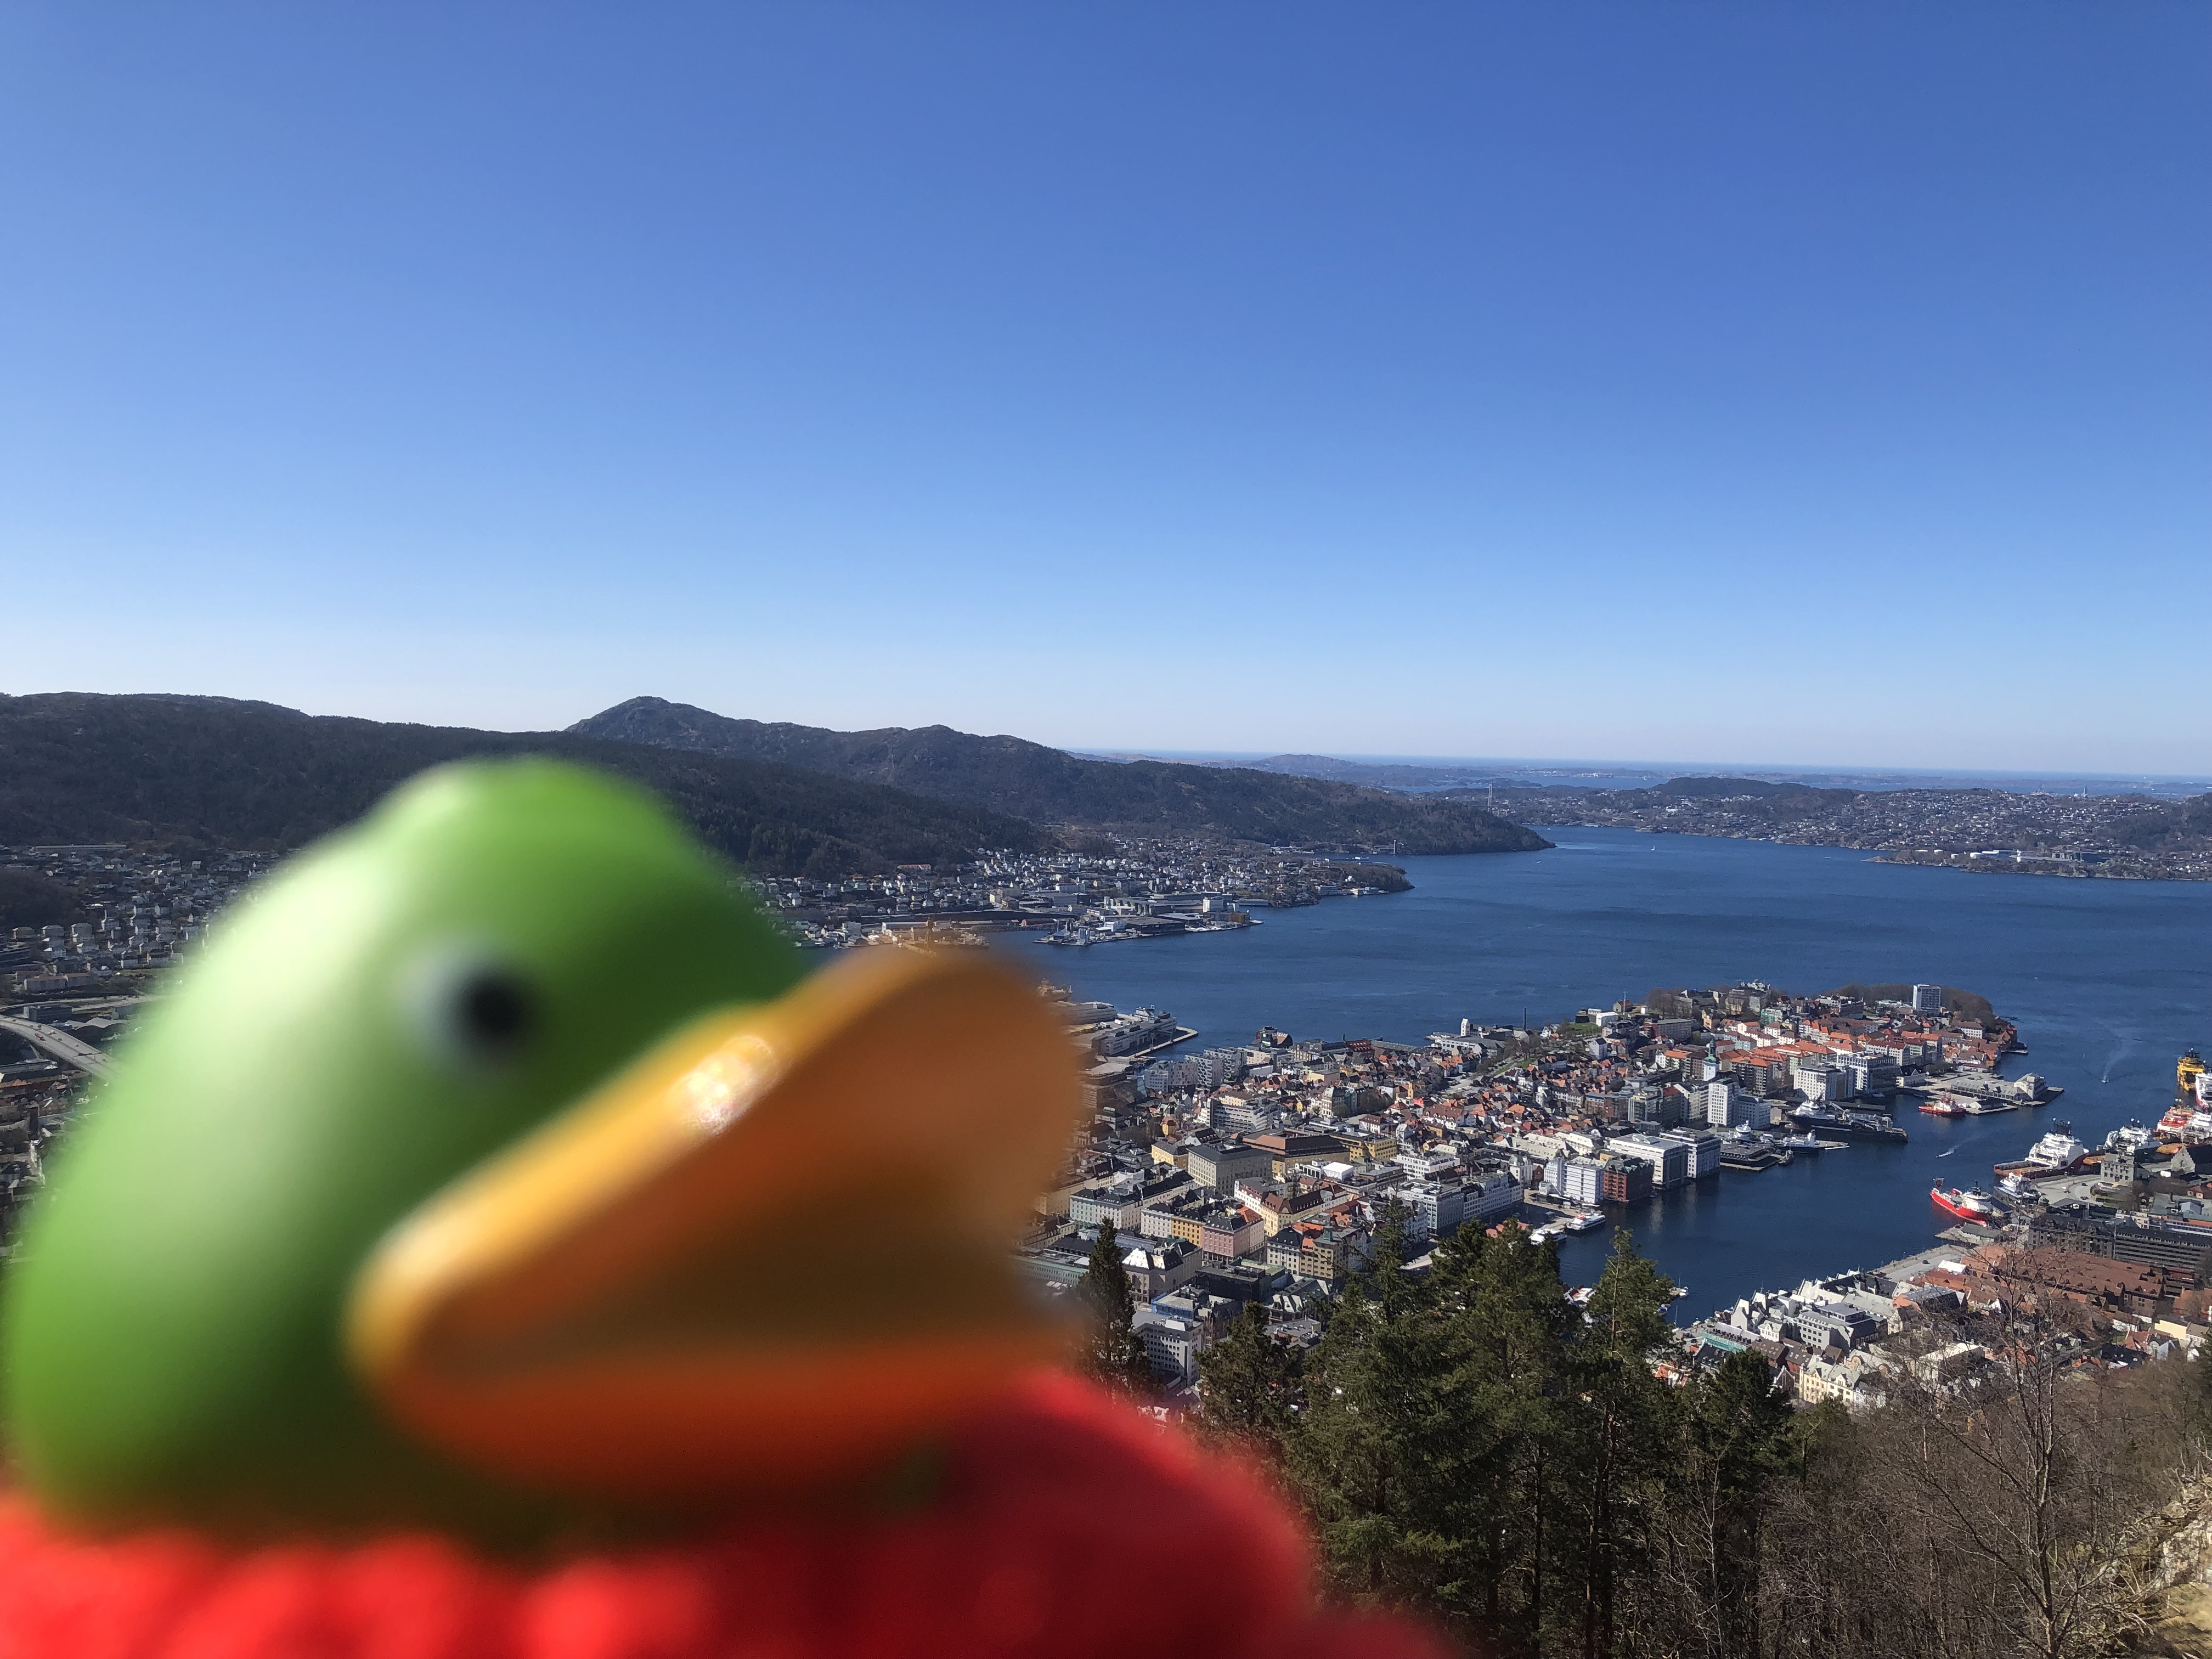
\includegraphics[height = 4.9cm]{images/guillaume10.jpg}
        \caption{Guillaume på Fløyen}
        \label{fig:guillaume10}
    \end{figure}
\end{frame}


